\PassOptionsToPackage{margin=1in}{geometry}
\documentclass[11pt]{article}
\usepackage{lmodern}
\usepackage{wordlike}
\usepackage{setspace}
\usepackage{pdfpages}
\usepackage{grffile}
\usepackage{graphicx}
\usepackage{fancyhdr}
\usepackage{indentfirst}
\usepackage{wrapfig}
\usepackage{amssymb}
\usepackage{amsmath}
\usepackage{geometry} % Required to change the page size to A4
\usepackage{float} % Allows putting an [H] in \begin{figure} to specify the exact location of the figure
\usepackage{hyperref} % Enables hyperlinks and text reference clicking
\usepackage{color} % Enables text font coloring
\usepackage{caption} 
\usepackage{subcaption} 

\pagestyle{fancy}
\lhead{CS 5714 UX Midterm Spring 2014}
\chead{}
\rhead{chris frisina}
\lfoot{Please redistribute as is or anonymized as you need}
\cfoot{}
\rfoot{\thepage \hspace{1 mm} fish}
\renewcommand{\headrulewidth}{0pt}
\renewcommand{\footrulewidth}{0pt}
% \doublespacing

\begin{document}

\title{CS 5714 UX Midterm Spring 2014}
\author{Chris Frisina}

\section*{Signature} % Q/A
  \begin{figure}[H]
  \centering
  
\includegraphics[height=0.9\linewidth]{img/signature.jpg}
  \caption{Pledge and signature}
  \label{fig:signature}
  \end{figure}

\section*{Part 1} % Q/A
  \begin{figure}[H]
  \centering
  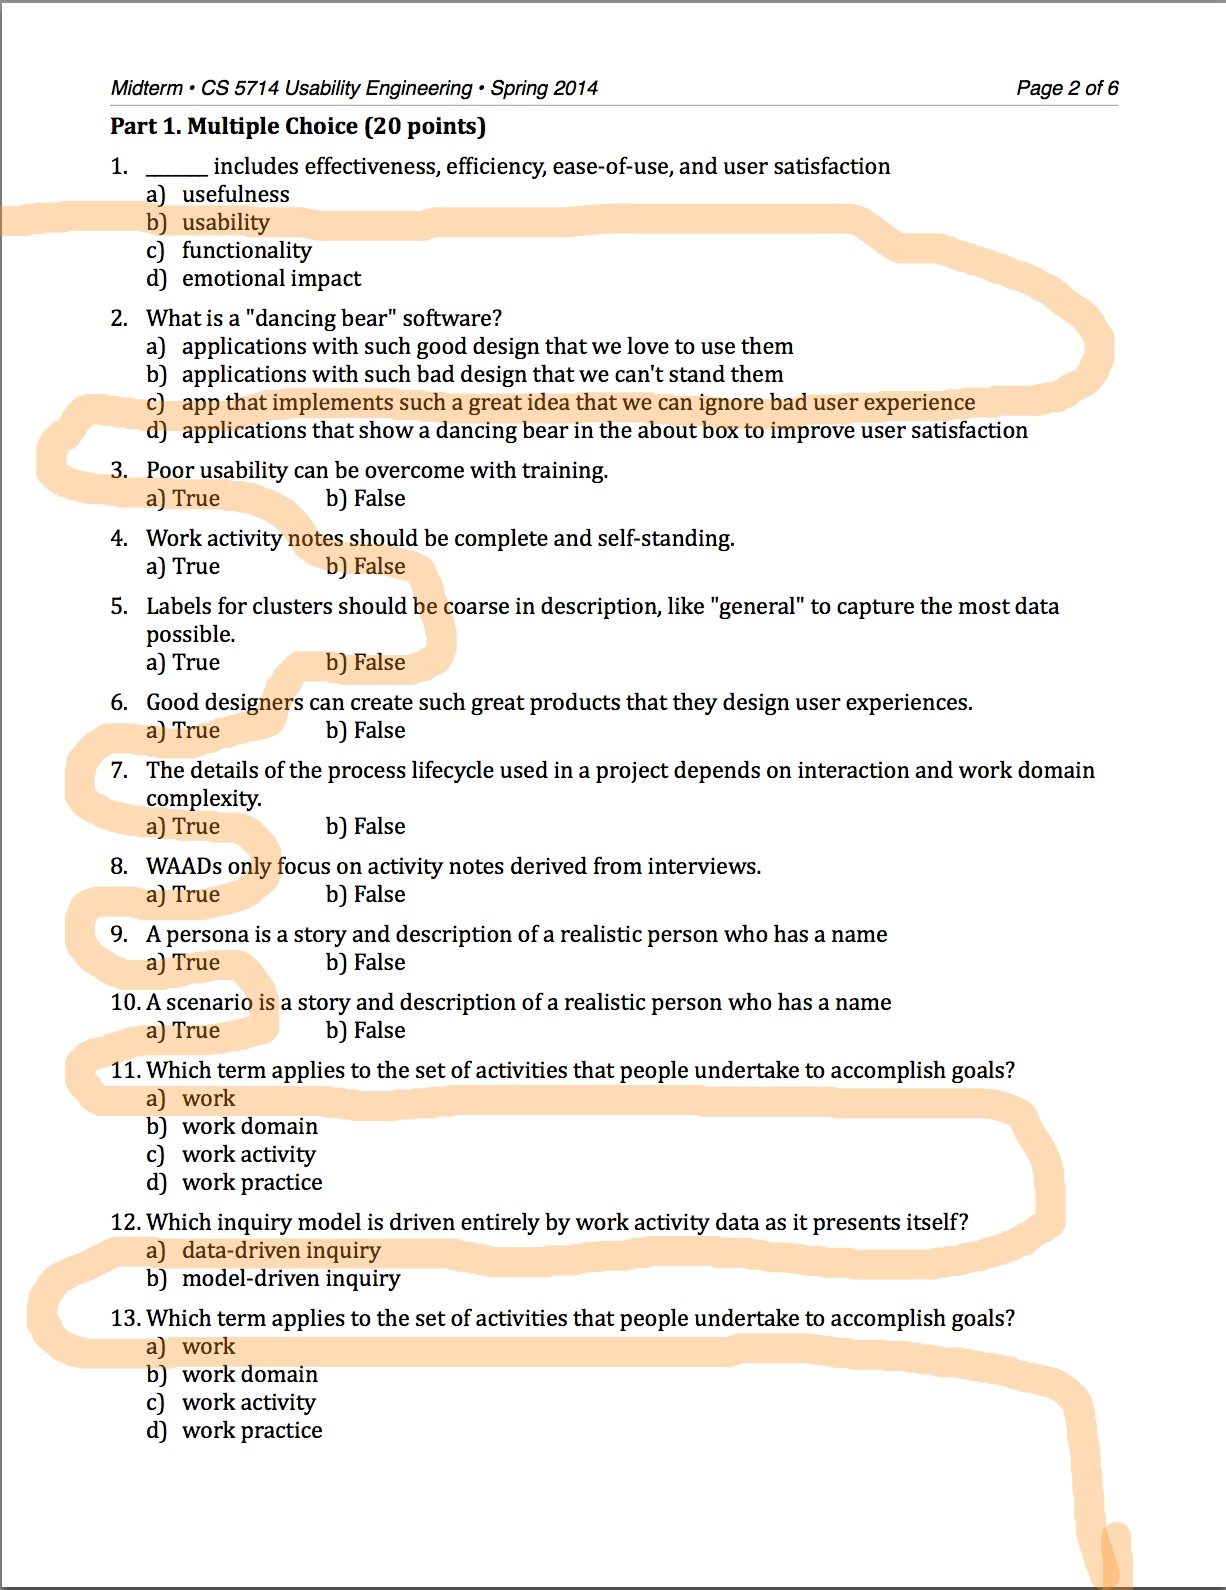
\includegraphics[height=0.9\linewidth]{img/one.jpg}
  \caption{Multiple Choice | True/False One}
  \label{fig:one}
  \end{figure}

  \begin{figure}[H]
  \centering
  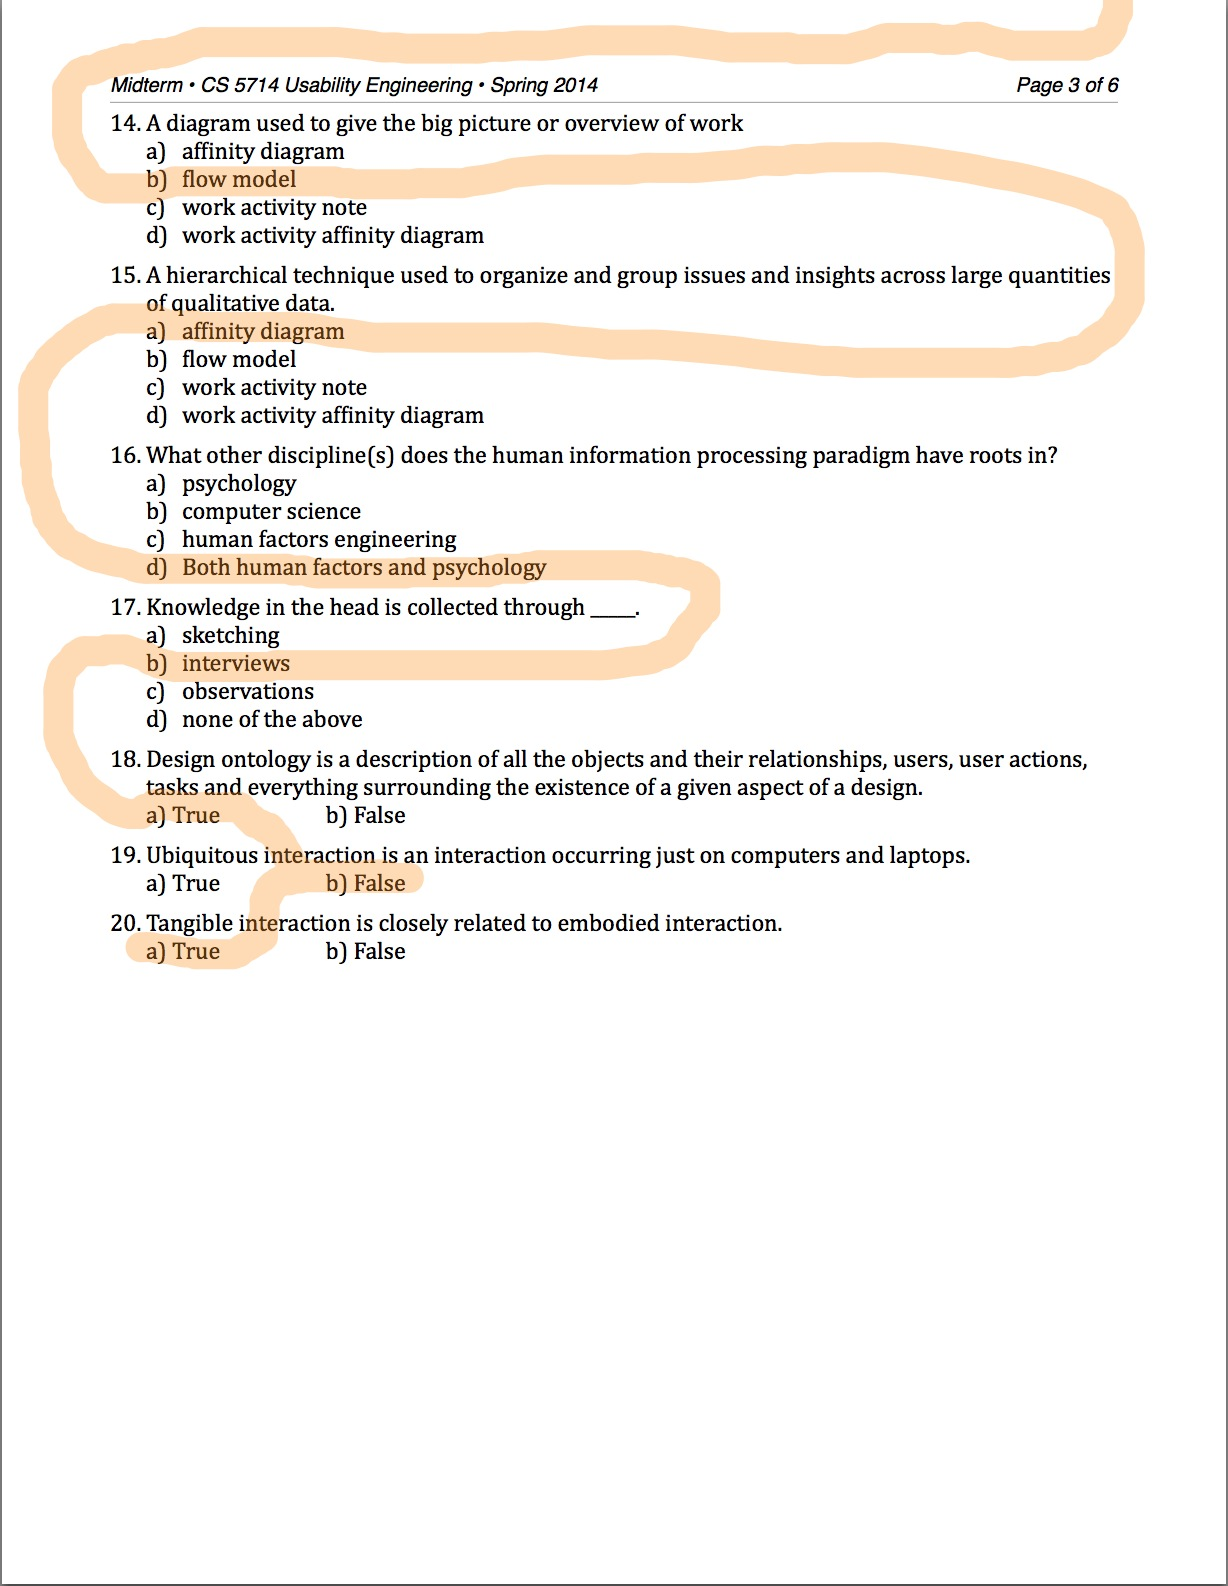
\includegraphics[height=0.9\linewidth]{img/two.jpg}
  \caption{Multiple Choice | True/False}
  \label{fig:two}
  \end{figure}


\section*{Part 2} % 1 page
  \subsection*{Question 1} 
  % (10 pts) Write a system concept statement for target systems above. This is a 100-to-150-word summary of the project, per the description of concept statement in the textbook and in our lectures. This is a high-level mission statement of a project—a synopsis or "boilerplate" description.  Include the name of the system, a description of the kinds of users expected, a brief statement of  what  users can do with it, and why it's useful (what problems  it  solves).  

  % What is the system name?  
  % –Who are the system users?  
  % –What will the system do? 
  % –What problem(s) will the system solve? (Be broad to include business objectives)
  % What is design vision and what are the emotional impact goals?
  % what experience will system provide to user
  % Audience broader than that of most other deliverables, including 
  % – Highlevel management 
  % – Marketing 
  % – Board of directors  
  % – Stockholders  
% – Even general public

  Graduate students at a large public educational institute have varying needs throughout their academic career.
  Their main contact is an overloaded faculty member who is struggling to accommodate all requests in a timely structured manner.

  I propose InkDrop, an automated proxy scheduler for assisting close community members in achieving meet-ups that last less than 5 minutes.
  While there are many communities that can benefit from InkDrop, it will initially support an academic community to accommodate rapidly changing multiplex organizational structures and process flows.
  All community members at some point require knowledge surrounding matriculation, and Inkdrop will help members access a centralized reference for decentralized content and information.
  Members will be able to navigate information flow charts to reduce unawareness, expedite the required paperwork flow, and take charge of their academic career while also aiding the faculty member in performing the job duties succinctly and expeditiously.

  143 words (not including this line of course)

  \subsection*{Question 2}
  % (20pts) Make  an  initial Flow model,  a “big  picture”  diagram of  the work  domain  and the entire  work  practice. Show  interconnections  among components  of  the work  domain. Show  work  Flow, information Flow, and all communications  among the components. Include non-human entities, such  as a central database  and non-computer communication Flow such as via email, telephone.
  Like all well executed User Experience Design processes, this is a first pass at the information provided.
  Subsequent interviews will include a discussion and verification about the physical representations of the current and proposed system and work flows.
  \begin{figure}[H]
  \centering
  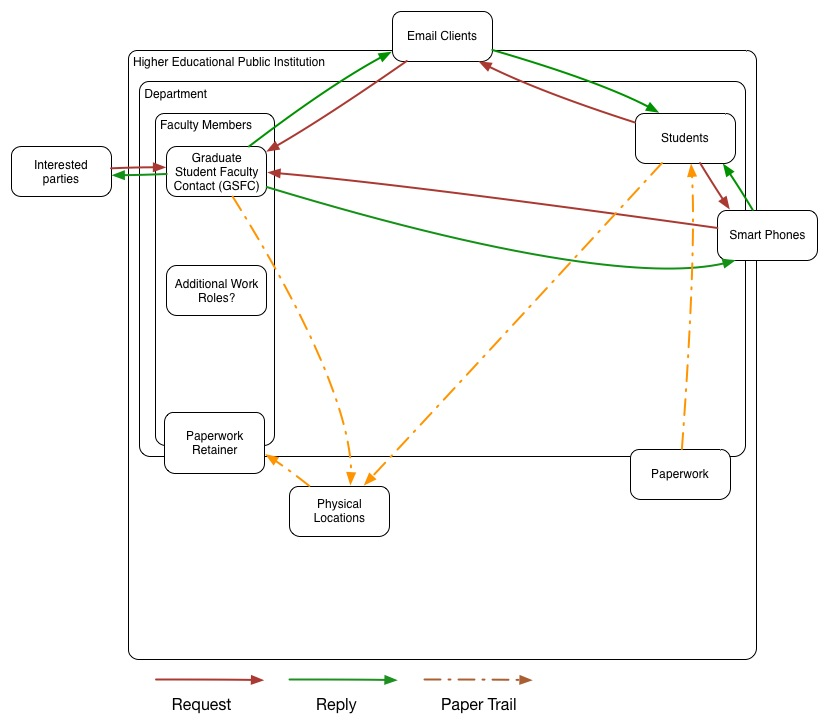
\includegraphics[height=0.9\linewidth]{img/workflow.jpg}
  \caption{Current Structure}
  \label{fig:current}
  \end{figure}


  \begin{figure}[H]
  \centering
  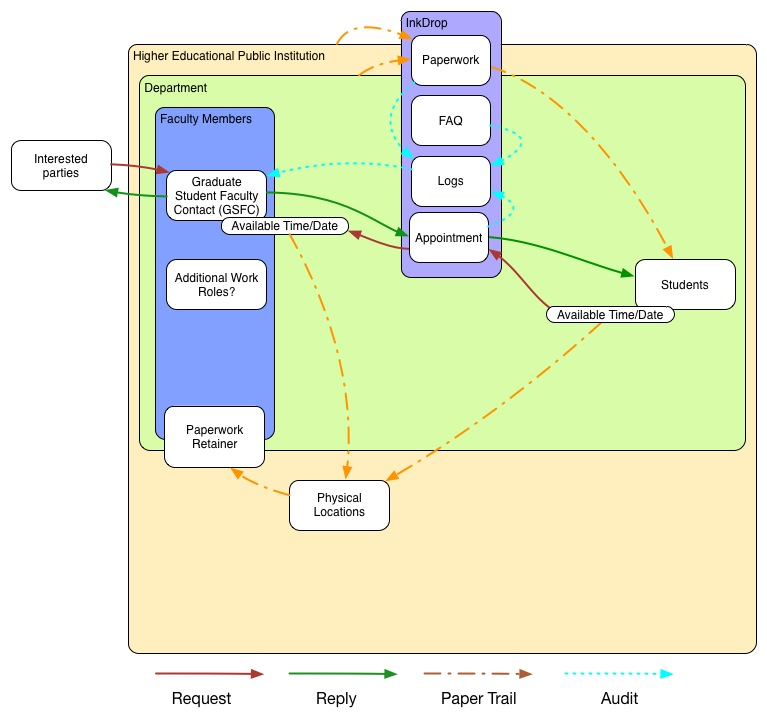
\includegraphics[height=0.9\linewidth]{img/workflow-proposed.jpg}
  \caption{Proposed Implementation}
  \label{fig:proposed}
  \end{figure}

  \subsection*{Question 3 - Work Roles}
  % . (20pts) Identify  all the work  roles in  the system  from  the interview transcript  above.  A work  role  is  deOined by  a corresponding job title or  a particular  type  of  work  assignment  or  a set of work  responsibilities. Work  roles don't always  involve using the system  being studied.  For each work  role, give  it  a name, and a brief description.
  Assumption: (Dr. MPQ @ a public institution) !== (Dr. Manuel @ VT) \&\& (Dr. MPQ) == (Benevolent Dictator):

  Roles marked with an asterisk (\**) are explicitly mentioned in the interview.
  Roles without an asterisk are inferred form the interview, however titles and duties have yet to be reified.
  \begin{description} % Numbered list example
  \item[Faculty Member \**]
  Dr. MPQ\\
  The roles and responsibilities of a faculty member are not mentioned
  \item[Graduate Student Faculty Contact (GSFC) \**]
  Dr. MPQ\\
  This role is in charge of helping graduate students in several capacities including signing paperwork, holding brief meetings, and consultation.
  It is unclear if these roles are independent of a formal work role title despite potentially having different purposes.
  Many of the concerns aside from signatures are centered around information communication.

  \item[Additional Work Roles \**]
  Dr. MPQ\\
  It is mentioned that he has many other work roles, but they are not explicitly discussed or delineated.

  \item[Paperwork Retainer, Interested parties]
  Unknown\\
  The paperwork flow is not clearly defined.
  For example, does the student(s) continue handling the paperwork, or the signature the final step.
  This leaves open the questions of who retains the paperwork, who views the paperwork aside from the student and GSFC

  \item[Student (s)]
  There are graduate students who need paperwork signed, consultation regarding graduation, and other questions surrounding their education.
  
  \end{description}

  There are also other roles that must be considered, but aren't easily classified as a work role given the lack of inquiry, but closer to places and domains that have influence on this particular client's case:
  \begin{description} % Numbered list example
    \item[Higher Educational Public Institution \**]
    Not known\\
    \item[Physical Locations \**]
    Campus, and KWII\\
    \item[Smart Phones, Email clients \**]
    While they are communication channels as well, they are explicitly different form a phone call, as they have physical components as well.
  \end{description}

  \subsection*{Question 4}
  % (20pts) Make  a hierarchical task inventory diagram showing the task structure for the product described in the interview. An HTI Diagram captures and catalogs the hierarchical  relationships among the tasks and subtasks that must be supported in the system. Remember that HTI does NOT capture temporal relationships.  
  \begin{figure}[H]
  \centering
  \includegraphics[height=0.9\linewidth]{img/task.jpg}
  \caption{InkDrop : Hierarchical task inventory diagram}
  \label{fig:task}
  \end{figure}

\section*{Part 3} % (10 points)
  % Discuss the following paper. Do not write more than one page. Make sure what you write are your own words, do not copy words from the paper. Also there are write-ups on the web summarizing this paper, they are easy to google. Do not use them. I am interested in your personal summary not a copy of words.  

  % In particular explain what is the third wave or the third paradigm presented on the paper and why it is important for the content of this course.

  Harrison, Tatar, and Sengers (HTS) identify a third paradigm of the HCI research area by first defining human factors then classical cognitivism/information processing.
  Their definition surrounds the strengthening of meaning based on interactions in particular situations.
  This view point is an HCI centered paradigm that tries to address the murky connection between symbols and referents in the common communication semantic triangle as in Figure \ref{fig:triangle}.

  \begin{wrapfigure}{HCI}{0.4\textwidth}
    \begin{center}
      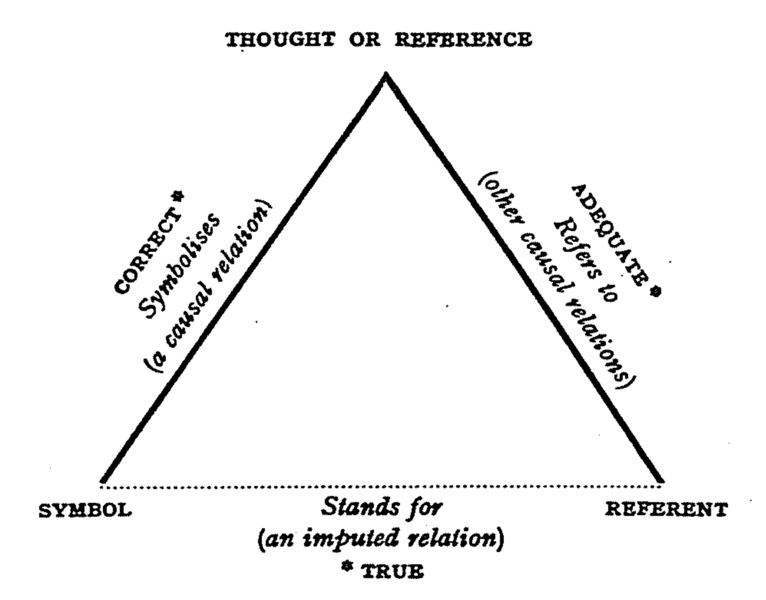
\includegraphics[width=0.38\textwidth]{img/semantic-triangle.png}
    \end{center}
    \caption{A traditional semantic triangle}
    \label{fig:triangle}
  \end{wrapfigure}
  I believe the strongest component of the this third phenomenologically-situated paradigm of understanding HCI is the importance of the user, in particular their domain knowledge and interactions in situations.
  As a challenge in designing any experience (electronic, situated, [inter/intra]-personal, or otherwise), accommodating varying viewpoints rarely occurs.
  The third paradigm stresses that the users' perceptions, knowledge, interactions, and should not be bijected and formally judged.
  This lack of adjudication is grounded around accommodating varying viewpoints and social structures, where precision can but infrequently exists.
  This lack of precision in the other two paradigms is ignored as being irrelevant.
  In the scope of the third paradigm, however, all contexts, experiences, and situations of every user are recognized and given weight.

  The requirement of the third paradigm to encompass situations, users, and viewpoints strengthens HCI as a field, especially relevant to user experience.
  This phenomenologically-situated idea is at a core of well rounded usability engineering principles and stages, in particular: participatory design, user inquiry, and evaluation methods.
  The third paradigm situates us designers and engineers to keep an open mind throughout the processes as we also try to concretize the connections that exist in the domains we are interacting with, while also understand our effect, similar to the \textit{entanglement} concerns proposed by Schrödinger in describing theoretical clashes among interpretations and experimentation.


% \section*{Bibliography}
\newpage

\end{document}